\documentclass[11pt,a4paper]{article}

\usepackage[margin=1in]{geometry}
\usepackage{lmodern}
\usepackage{amsthm}
\usepackage[section]{placeins}
\usepackage[font=small,labelfont=bf]{caption}
\setlength{\parindent}{0pt}
\setlength{\parskip}{0.5em}
\linespread{1.06}
\renewcommand{\abstractname}{Overview}

\usepackage[T1]{fontenc}
\usepackage{microtype}
\usepackage{amsmath,amssymb}
\usepackage{booktabs,tabularx,array,multirow}
\usepackage{graphicx}
\usepackage[dvipsnames]{xcolor}
\usepackage{cite}
\usepackage{url}
\usepackage[hidelinks]{hyperref}
\usepackage[nameinlink,capitalise]{cleveref}

\crefname{figure}{Fig.}{Figs.}
\Crefname{figure}{Fig.}{Figs.}
\crefname{table}{Table}{Tables}
\Crefname{table}{Table}{Tables}
\crefname{section}{Section}{Sections}
\Crefname{section}{Section}{Sections}
\crefname{subsection}{Section}{Sections}
\Crefname{subsection}{Section}{Sections}
\crefformat{equation}{(#2#1#3)}
\Crefformat{equation}{Equation~(#2#1#3)}
\crefrangeformat{equation}{(#3#1#4)--(#5#2#6)}

\newtheorem{definition}{Definition}
\newtheorem{proposition}{Proposition}
\newtheorem{corollary}{Corollary}
\crefname{definition}{Definition}{Definitions}
\crefname{proposition}{Proposition}{Propositions}
\crefname{corollary}{Corollary}{Corollaries}

\newcolumntype{Y}{>{\raggedright\arraybackslash}X}
\newcolumntype{P}[1]{>{\raggedright\arraybackslash}p{#1}}
\newcommand{\true}{\textsc{true}}
\newcommand{\false}{\textsc{false}}
\newcommand{\unknown}{\textsc{unknown}}

\graphicspath{{figures/}}
\newcommand{\repositoryurl}{https://github.com/fishOmlette/X}

\hypersetup{
  pdftitle={When Does Predicting Failure Help? A Boundary Analysis of Predictive versus Reactive Runtime Assurance for Multi-Robot Coordination},
  pdfauthor={Mohamed Adil Farukh},
  pdfkeywords={runtime assurance, multi-robot systems, predictive monitoring, safety margins, time to collision, reproducible evaluation}
}

\begin{document}

\title{When Does Predicting Failure Help?\\[0.4em]
  \large A Boundary Analysis of Predictive versus Reactive Runtime Assurance
  for Multi-Robot Coordination}

\author{Mohamed~Adil~Farukh\\[0.3em]
  \small\href{mailto:mdadilfarooq@gmail.com}{mdadilfarooq@gmail.com}}
\date{}

\maketitle

\begin{abstract}
A prediction can tell a robot to act before a safety margin runs out.  But a
fixed threshold can also make it act early.  I wanted to understand when
prediction adds something beyond choosing a more conservative threshold.  I
study this question with a simplified timing model and two kinematic simulation
setups, giving both rules the same tuning budget and testing on separate noise
seeds.

In the timing model, the predictive rule is a current-margin threshold whose
buffer scales with the estimated rate of decline.  Extra lead changes the
recovery outcome only within a band set by recovery duration and deadline
slack; old observations consume that lead one for one.  The minimal predictive
horizon wastes less lead than the minimal safe fixed buffer when recovery
needs a similar amount of time across cases but the corresponding margins
differ, provided the rates can be estimated.

The clearest gain appears in the three-robot shared-zone test.  Both tuned
rules succeed in all 1,620 conflict episodes, and prediction reduces mean
completion time by $2.78$\,s (paired 95\% bootstrap interval
$[2.66,2.90]$\,s).  On clear paths, it reduces unnecessary serializations from
1,080 to 21 out of 1,620 episodes.  The two-robot test exposes a different
behavior: the tuned fixed rule records no collisions in 6,750 conflict episodes
and prediction records two.  Together, the tests show where adapting the margin
helps in these simulations and where estimating its rate becomes the weak point.
\end{abstract}

\noindent\textbf{Keywords:} Runtime assurance, multi-robot systems, predictive
monitoring, safety margins, time to collision, reproducible evaluation.

\section{Introduction}
\label{sec:introduction}

\IEEEPARstart{A}{utonomous} systems increasingly rely on runtime layers that
monitor safety, performance, or mission properties and intervene during
execution.  Examples include modular runtime assurance for robotics
\cite{desai2019soter}, mission-level runtime assurance for autonomous driving
\cite{tsai2026missionrta}, compositional runtime verification for robot swarms
\cite{kekatos2026swarmrta}, and predictive runtime verification, enforcement,
and monitoring
\cite{pinisetty2017prv,pinisetty2017pre,yoon2019prm,wheatman2021radics}.
Prediction is attractive because the extra lead it provides may allow a recovery
that preserves the mission instead of an emergency stop.

A predictive monitor is, however, an inference component inside the robot's
decision cycle.  It must estimate how fast a margin is degrading from noisy and
possibly delayed observations, run within the cycle's latency budget, and be
tuned and certified like any other safety function.  A reactive rule can also
intervene early: it only needs a larger fixed margin.  Comparing a predictor
with an unpadded reactive trigger therefore does not show that prediction is
necessary.  The fair comparison gives the fixed margin a comparable tuning
budget.  We ask: \emph{when does predicting the loss of feasibility outperform
reacting to it?}

\Cref{sec:analysis} answers this question within an idealized timing model.  A
trigger that fires when the projected time to margin expiry falls below a
horizon is a reactive trigger with a rate-scaled margin.  An earlier trigger
changes a recovery outcome only within a band set by recovery duration and
deadline slack, and observation age shrinks that band exactly as lost lead does.
The minimal predictive horizon wastes less lead than the minimal safe fixed pad
when recovery requires a similar lead in every case but, because degradation
rates differ, a different margin.  \Cref{sec:method,sec:results} examine these
conditions in controlled simulations.  Exploratory sweeps locate the boundary,
and two further evaluations separate tuning from testing.  In the held-out
single-margin comparison, the tuned fixed rule records $0/6750$ conflict
collisions and the tuned predictive rule records $2/6750$, so the outcomes do not
support an efficiency comparison.  In a three-robot study with genuinely
conflicting geometry and an explicit serialization state machine, both tuned
rules succeed in every held-out conflict episode, and the predictive rule has a
shorter mean makespan on the fixed scenario grid.

The paper makes four contributions:
\begin{enumerate}
  \item a reduction showing that the studied horizon-based predictive trigger is
    a rate-adaptive current-margin threshold (\cref{prop:reduction});
  \item a boundary condition, in terms of recovery duration, deadline slack, and
    observation age, for when added lead changes the recovery outcome
    (\cref{prop:boundary,cor:age}), and a characterization of when the minimal
    predictive horizon wastes less lead than the minimal safe fixed pad
    (\cref{prop:homogeneity});
  \item a reproducible evaluation protocol that separates exploratory in-sample
    sweeps from seed-disjoint tuning and testing, gives both rules equal tuning
    budgets, reports failures before timing, and withholds timing inference when
    failure outcomes differ; and
  \item a genuine-conflict three-robot evaluation with explicit approaching,
    waiting, crossing, and cleared states, which identifies a one-shot
    serialization regime in which the rate-adaptive trigger shortens completion
    time relative to the tuned fixed pad at matched observed outcomes.
\end{enumerate}

The paper characterizes a trigger mechanism rather than proposing a controller.
The experiments are stylized two-dimensional kinematic simulations chosen to
isolate that mechanism, and the results apply only to the tested models.
\Cref{sec:limitations} details these limits.

\section{How this connects to prior work}
\label{sec:related}

\emph{Predictive runtime verification and enforcement.}  Predictive runtime
verification uses a priori knowledge of the system to reach a conclusive verdict
before the observed execution alone permits one \cite{pinisetty2017prv}, and
predictive runtime enforcement reduces to non-predictive enforcement when no
such knowledge is available \cite{pinisetty2017pre}.  For stochastic linear
systems, Yoon \emph{et al.}\ determine whether a control sequence exists over a
finite horizon that maintains a safety property with sufficiently high
probability \cite{yoon2019prm}.  RADICS combines a black-box monitor that
switches to a safe algorithm on a failing trajectory with a white-box monitor
that predicts such trajectories earlier \cite{wheatman2021radics}.  Predictive
safety filters solve an online finite-horizon problem to certify or modify a
proposed input under model uncertainty \cite{wabersich2021filter}.  I ask a
narrower comparative question: once recovery timing and a tuned current-margin
threshold are included, when does an earlier trigger change the measured
outcome?

\emph{Runtime-assurance architectures.}  Simplex uses a simple, reliable core to
bound the behavior of more complex functionality \cite{sha2001simplex}.  Its
black-box extension uses runtime checks to transfer control between advanced and
baseline controllers and includes a multi-robot case study
\cite{mehmood2022blackbox}, and SOTER composes robotics runtime-assurance modules
that switch between advanced and safe controllers \cite{desai2019soter}.
Mission-level monitors can reject commands that would make a mission infeasible
before they execute \cite{tsai2026missionrta}; compositional monitoring can
detect policy violations that emerge only across a robot swarm
\cite{kekatos2026swarmrta}; and collective run-time adaptation addresses safety
and mission completion in multi-robot systems \cite{bozhinoski2019collective}.
These works design what happens after a trigger.  I study the trigger rule
itself: a projected time to threshold versus a fixed current-margin threshold.

\emph{Adaptive margins and time-to-threshold triggers.}  Time to collision, the
ratio of range to closing speed, has long been used to time braking and to grade
traffic conflicts \cite{lee1976ttc,mahmud2017surrogate}.
\Cref{prop:reduction} is the corresponding observation for a generic monitored
margin: a threshold on projected time is a threshold on the margin scaled by the
estimated rate.  Adaptive margins can also scale a safety buffer with relative
speed, braking capability, and prediction uncertainty \cite{xu2026raam}, and
control barrier functions provide a broader framework for encoding and enforcing
safety constraints \cite{ames2019cbf}.  Because the horizon trigger studied here
is one particular rate-scaled margin, it should be compared with tuned fixed
margins and not only with an unpadded threshold.

\emph{Prognostics and recoverability.}  Prognostics estimates whether and when
faults will occur in order to inform condition-based maintenance
\cite{jardine2006prognostics}.  Runtime-assurance verification formalizes the
adequacy of decision timing and time-bounded recoverability
\cite{nigam2023recoverability}.  Recent work on adaptive governance of AI agents
predicts when a viability index will cross its boundary from a first-order fit
of its recent trend \cite{marin2026governance}.  These results motivate a
point-of-no-return analysis, but they do not by themselves establish when an
earlier trigger beats a tuned fixed margin for a robot model.

\section{Problem Setup}\label{sec:setup}

Let a scalar margin $M(t)\in\mathbb{R}$ summarize remaining mission feasibility, with $M(t)\ge 0$ defining the monitored feasible set and $M(t)=0$ its boundary. During the degradation phase of interest, a fault drives the margin downward, and
\[
  t_0=\inf\{t:M(t)\le 0\}
\]
denotes expiry of the positive margin, by first contact with or crossing of the boundary. All infima are over the monitored time domain, with $\inf\varnothing=+\infty$; for the timing analysis we assume that $t_0$ is finite and attained. Let $t_f$ be the physical deadline by which a recovery must have taken effect. We assume here that the monitored margin is conservative enough that $t_f\ge t_0$, and define the post-expiry slack $\delta=t_f-t_0\ge0$.

A recovery triggered at $t_{\mathrm{trig}}$ requires duration $\tau_r>0$ and succeeds if
\begin{equation}\label{eq:success}
  t_{\mathrm{trig}}+\tau_r\le t_f.
\end{equation}
Equivalently, $t_{\mathrm{pnr}}=t_f-\tau_r$ is the latest safe trigger time, or point of no return for that recovery.

We compare two trigger policies. A fixed-margin reactive policy fires when
\[
  t_{\mathrm{trig}}=\inf\{t:M(t)\le\rho\},
\]
where $\rho\ge0$ is a fixed pad, in the same units as $M$. The predictive policy estimates the degradation rate $\hat r(t)=-\widehat{\dot M}(t)$ and, when that estimate is positive, fires when projected time-to-expiry is at most a time horizon $T_h\ge0$:
\begin{equation}\label{eq:pred}
\begin{aligned}
  t_{\mathrm{trig}}
  &=\inf\Bigl\{t:M(t)\le0\ \lor \\
  &\qquad [\hat r(t)>0\ \land\ M(t)/\hat r(t)\le T_h]\Bigr\} \\
  &=\inf\Bigl\{t:M(t)\le0\ \lor \\
  &\qquad [\hat r(t)>0\ \land\ M(t)\le T_h\hat r(t)]\Bigr\}.
\end{aligned}
\end{equation}
An unavailable or non-positive rate estimate therefore leaves only the unpadded current-margin condition $M(t)\le0$.

\section{Analysis}\label{sec:analysis}

\begin{proposition}[Predictive triggering is a rate-scaled margin]\label{prop:reduction}
On its positive-rate branch, the predictive rule in \eqref{eq:pred} is a reactive threshold with the time-varying pad $\rho(t)=T_h\hat r(t)$; its fallback pad is zero. Suppose that, on a monitored interval containing both threshold crossings, $M(t)=r(t_0-t)$ with an exact constant estimate $\hat r=r>0$, and that monitoring begins before either crossing. The predictive rule then fires $T_h$ seconds before $t_0$, while a fixed pad $\rho$ fires $\rho/r$ seconds before $t_0$. Thus, at one known constant rate, the fixed pad $\rho=T_h r$ reproduces the predictive trigger exactly. For a positive horizon and two distinct rates, no one fixed pad provides that same constant positive lead time at both rates.
\end{proposition}
\begin{proof}
The threshold identity on the positive-rate branch follows directly from \eqref{eq:pred}. Under the stated affine model, $M(t_0-L)=rL$. The predictive threshold $M=T_h r$ is therefore reached at $L=T_h$, and the fixed threshold $M=\rho$ at $L=\rho/r$; the monitoring assumption makes these the first threshold crossings. If $T_h>0$ and $r_1\ne r_2$, matching that lead at both rates would require both $\rho=T_h r_1$ and $\rho=T_h r_2$, which is impossible.
\end{proof}

\begin{proposition}[When lead time changes the recovery outcome]\label{prop:boundary}
Assume a predictive rule triggers $L\ge0$ seconds before $t_0$, while the unpadded reactive rule triggers at $t_0$. Then:
\begin{enumerate}
  \item if $\tau_r\le\delta$, both rules recover in time;
  \item if $\delta<\tau_r\le\delta+L$, only the predictive trigger recovers in time; and
  \item if $\tau_r>\delta+L$, neither rule recovers in time.
\end{enumerate}
\end{proposition}
\begin{proof}
By \eqref{eq:success}, the unpadded rule succeeds exactly when $t_0+\tau_r\le t_f$, or $\tau_r\le\delta$. The predictive rule succeeds exactly when $t_0-L+\tau_r\le t_f$, or $\tau_r\le\delta+L$. The three cases follow.
\end{proof}

\begin{corollary}[Necessary conditions for an advantage over fixed pads]\label{cor:factors}
Within the deadline-only model of Proposition~\ref{prop:boundary}, an earlier predictive trigger turns a recovery failure into success only in the middle band, which requires positive lead. Within the affine, exact-rate model of Proposition~\ref{prop:reduction}, a positive-horizon predictor can have a structural advantage over a \emph{single fixed pad across cases} only if the degradation rates vary: at one known constant rate, an equivalent fixed pad exists. These conditions are necessary within the stated models, not sufficient; estimation error and the joint distribution of rates, slack, and recovery times can still make a fixed pad preferable.
\end{corollary}

Figure~\ref{fig:mech} illustrates the timing argument.

\begin{figure}[tbp]
\centering
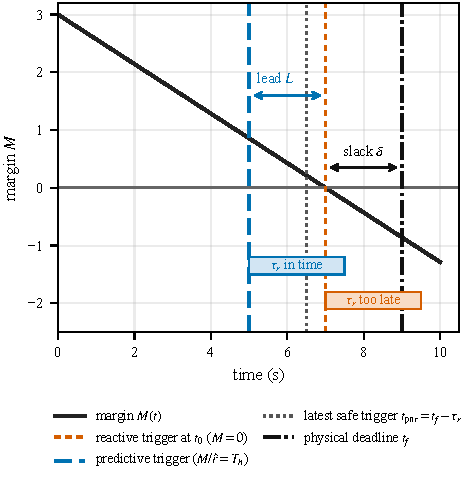
\includegraphics[width=0.72\linewidth]{fig_mechanism.pdf}
\caption{The unpadded reactive rule fires at margin expiry, while the predictive rule fires $L$ seconds earlier. The earlier trigger changes the recovery outcome only when $\delta<\tau_r\le\delta+L$.}
\label{fig:mech}
\end{figure}

\section{Evaluation Methodology}
\label{sec:method}

\subsection{Single-Margin Simulator}

Two robots travel on perpendicular paths through one crossing, and robot A may
brake and wait for robot B.  The monitored margin is a time headway,
$M=\lvert\hat g\rvert-k_\sigma\sigma-G_{\mathrm{safe}}$, where $\hat g$ is the
estimated difference between the arrival times of B and A at the crossing,
$\sigma$ is a range-dependent uncertainty allowance, and
$G_{\mathrm{safe}}=0.5$\,s is the required headway; additive Gaussian noise
perturbs each measurement.  An optimistic hidden bias $s f^{p}$ delays B's
estimated arrival, where $s$ is the fault severity in seconds, $f\in[0,1]$ is
B's remaining range fraction, and the exponent $p$ sets how the bias decays:
$p<1$ reveals the conflict late, $p=1$ linearly, and $p>1$ early.  Recovery is
rate-limited braking with capability $a_{\max}$.  The predictive rule estimates
the margin slope with the Theil--Sen estimator \cite{sen1968theilsen} over the
eight most recent samples.  To avoid dividing by a fitted slope near zero, it
projects only when the fitted decay exceeds $10^{-3}$ margin units per second
($10^{-6}$ in the coordination simulator) and otherwise uses its $M\le0$
fallback.

Two model-specific quantities bound the latest useful trigger; neither is a
general safety certificate.  A continuous-time braking calculation gives the
latest trigger that stops A outside the wider crossing zone, $8.65$\,s with the
default parameters; it is conservative relative to the simulator's collision
condition.  Deterministic replay on the simulator's $0.1$\,s control grid finds
$8.8$\,s as the latest tested forced-trigger time that avoids a collision in the
default conflict episode; this boundary is empirical and grid-dependent.

\subsection{Three-Robot Coordination Simulator}

Three robots approach one shared zone at a nominal speed of $1.2$\,units/s; the
zone is one unit long, so the nominal occupancy is $0.83$\,s.  In the conflict
condition, start distances of $(12,12.5,13)$ units put adjacent nominal entry
times only $0.42$\,s apart, so untreated trajectories overlap physically.  In the
clear condition, start distances of $(12,14,16)$ units separate entries by
$1.67$\,s.  A collision is recorded when interpolated zone-occupancy intervals
overlap, and a separate headway violation when two entry times are less than
$5/6$\,s apart.  Each robot's estimated arrival time includes a decaying hidden
bias with per-robot multipliers $(0,1,2)$ and the exponent family used above.
For each pair of robots, the monitored margin is the absolute difference between
their estimated arrival times, minus the required headway and both uncertainty
allowances, plus measurement noise.  The fixed rule triggers when any pairwise
margin is at most $\rho$.  The predictive rule keeps a separate Theil--Sen slope
history for each pair and triggers when a margin is nonpositive or its projected
time to zero is at most $T_h$.

Both rules invoke the same recovery, an explicit one-shot serialization state
machine.  Robots start in the \textsc{approaching} state.  At the first trigger,
any robot already \textsc{crossing} is placed first, the others are ordered by
their current estimated arrival times, and the order is committed for the
episode.  Every later robot enters \textsc{waiting} with all earlier robots as
blockers and returns to \textsc{approaching} only after every blocker is
\textsc{cleared}.  Pairwise slope histories are reset at commitment, and no robot
yields twice.  The design isolates the effect of trigger timing on a fixed
recovery; it is not a general multi-robot planner.  \Cref{tab:parameters} lists
the main parameters of both simulators.

\begin{table}[!t]
  \centering
  \caption{Simulator and Evaluation Parameters}
  \label{tab:parameters}
  \footnotesize
  \setlength{\tabcolsep}{4pt}
  \begin{tabular}{@{}lll@{}}
    \toprule
    Parameter & Single margin & Coordination \\
    \midrule
    Robots & 2 & 3 \\
    Time step & $0.1$\,s & $0.1$\,s \\
    Nominal speed & $1.2$\,units/s & $1.2$\,units/s \\
    Required headway & $0.5$\,s & $5/6$\,s \\
    Measurement-noise s.d. & $0.05$\,s & $0.05$\,s \\
    Slope window & 8 samples & 8 samples \\
    $a_{\max}$ (units/s$^2$) & $0.5,1.0,2.5$ & $0.5,1.0,2.5$ \\
    Degradation exponent $p$ & $0.7,1.0,1.5$ & $0.7,1.0,1.5$ \\
    Fault severity $s$ (s) & $2,4,6,8,10$ & $2,6,10$ \\
    Conflict scenarios & 45 & 27 \\
    Pad and horizon grid & $0$--$4$, step $0.25$ & $0$--$4$, step $0.25$ \\
    Tuning / test replicates & 25 / 150 & 20 / 60 \\
    Held-out conflict episodes & 6,750 per arm & 1,620 per arm \\
    \bottomrule
  \end{tabular}
\end{table}


\subsection{Evaluation Protocol}

\emph{Exploratory sweeps.}  The dose-response experiment compares an
uncertainty-blind arrival-gap trigger, the current-margin trigger at $M=0$, and
the predictive rule with $T_h=2.0$\,s, using 40 paired noise seeds at each of
seven severities.  The recovery-capability and degradation-shape sweeps use 25
paired seeds at each of five severities, or 125 episodes per plotted setting and
rule; the shape sweep fixes $a_{\max}=0.8$.  For each setting, the fixed-pad
candidates are $\rho\in\{0,0.5,1.0,1.5,2.0,2.5,3.0,4.0\}$\,s, and the displayed
comparator is the candidate with the lowest mean successful elapsed time among
those for which every episode succeeds on the same setting and seed grid.
Selection and reporting therefore use the same simulations, so these figures are
mechanism checks rather than out-of-sample estimates.

\emph{Seed-disjoint single-margin evaluation.}  The evaluation crosses three
recovery capabilities, three degradation exponents, and five severities, giving
the 45 conflict scenarios of \cref{tab:parameters}.  The fixed pad and the
predictive horizon are both searched from $0$ to $4$ in steps of $0.25$.  Each
candidate receives 25 tuning replicates per scenario (1,125 episodes).  Among
candidates with no tuning collision, selection minimizes the mean conflict
elapsed time and breaks ties toward the smaller parameter.  Testing then uses
150 new replicates per scenario, or 6,750 episodes per conflict arm.  Clear-path
behavior is evaluated at $a_{\max}=1.0$ over the 15 exponent--severity
combinations, for 2,250 episodes per arm; a yield in this condition is a false
yield.  The original $T_h=2.0$\,s rule is retained as a diagnostic arm, but the
primary comparison uses the separately tuned horizon.

\emph{Seed-disjoint coordination evaluation.}  Tuning crosses the same three
capabilities and exponents with three severities, giving 27 scenarios, and
searches both parameters over the same grid.  Each candidate receives 20 tuning
replicates per scenario (540 episodes).  A candidate qualifies only if every
tuning episode reaches the exit without collision, headway violation, timeout,
or serialization breach; selection minimizes the mean successful makespan and
breaks ties toward the smaller parameter.  Each selected rule and a
no-intervention reference then receive 60 new replicates per scenario and
condition, or 1,620 episodes.

\emph{Seeds.}  Every split--scenario--replicate tuple maps to a distinct
deterministic seed, giving 10,125 single-margin and 3,780 coordination seeds
with no overlap between tuning and testing.  A tuple's seed is shared across
candidates and rules to preserve pairing.  The split therefore holds out noise
realizations only; the simulators and scenario grids remain fixed.

\subsection{Statistical Reporting}

Failure counts are reported before any timing comparison.  For each exact
scenario, we compute a two-sided 95\% Wilson score interval for the collision
probability \cite{wilson1927}.  We report the largest upper endpoint across the
pointwise intervals; this maximum is neither a simultaneous confidence bound nor
an estimate for a population of scenarios, and pooled counts summarize a fixed
factorial design rather than one homogeneous binomial experiment.  Elapsed time
and makespan are summarized only over successful episodes.  A paired percentile
bootstrap with 20,000 resamples, clustered by test replicate
\cite{efron1993bootstrap}, is computed only when every compared pair succeeds.
If failure outcomes differ, we report descriptive successful-only means and
suppress the inferential timing comparison.

\subsection{Connection to the Timing Model}

The recovery-capability sweep varies $a_{\max}$ as a proxy for recovery
duration, and the exponent sweep varies how quickly the margin degrades.  The
simulations do not measure the episode-level distributions of $\tau_r$,
$\delta$, $L$, and $\Delta$, and they introduce no observation delay.  They test
behavior consistent with the timing argument but do not validate
\cref{prop:boundary,prop:homogeneity} by measuring all of their variables.

\section{Results}
\label{sec:results}

\subsection{Exploratory Sweeps}

\emph{Untuned baselines favor early triggering (\cref{fig:dose}).}  Against an
uncertainty-blind arrival-gap rule and an unpadded current-margin rule, the
predictive rule with $T_h=2.0$\,s appears strong.  With rate-limited recovery
($a_{\max}=1.0$), the uncertainty-blind rule fails first as severity grows, the
unpadded rule collides in many moderate- and high-severity episodes, and the
predictive rule records no collision on this exploratory seed grid.  Earlier
action can therefore matter in the simulator, but this does not show that
prediction is needed, because a padded current-margin rule can also act early.

\begin{figure}[!t]
  \centering
  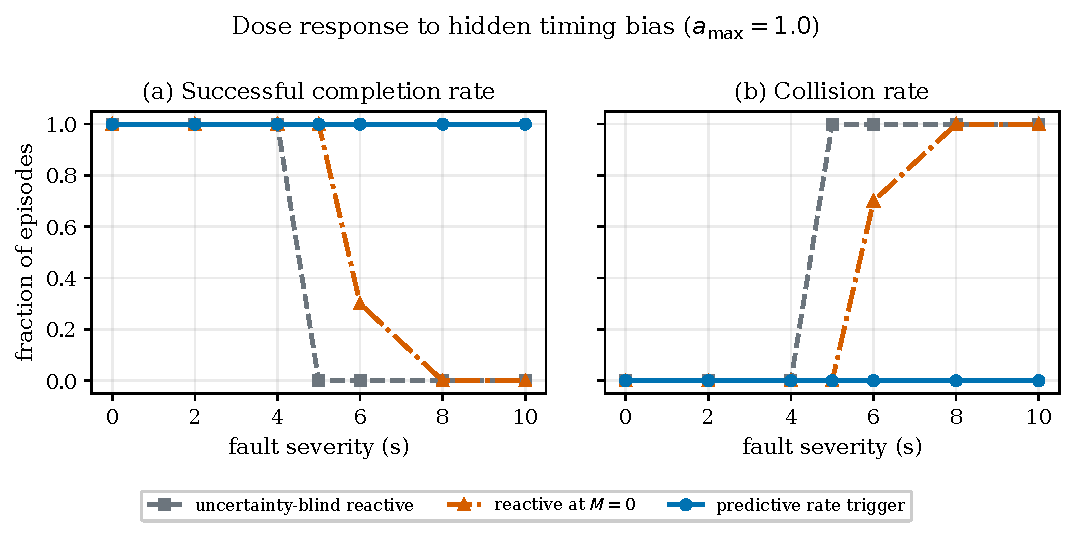
\includegraphics[width=\columnwidth]{fig_dose.pdf}
  \caption{Exploratory single-margin dose response with $T_h=2.0$\,s and
  $a_{\max}=1.0$: (a) successful completion rate and (b) collision rate over 40
  paired noise seeds per severity.  \Cref{fig:boundary} adds an in-sample
  fixed-pad comparator.}
  \label{fig:dose}
\end{figure}

\emph{The observed boundary is narrow (\cref{fig:boundary}).}  The plotted
difference is the mean elapsed time of the selected fixed pad minus that of the
predictive rule, so positive values favor prediction, and the fixed pad is
selected in-sample at every setting.  Under the slowest recovery
($a_{\max}=0.5$), the predictive rule finishes about $0.56$\,s sooner; the sign
changes as recovery becomes faster, reaching $-1.31$\,s at $a_{\max}=3.0$.  In
the degradation-shape sweep, the predictive rule records collisions at $p=0.3$
and $p=0.5$, where no tested fixed pad succeeds in every episode either; it is
about $1.23$\,s faster at $p=0.7$ and slower than the selected fixed pad from
$p=0.9$ onward.  These differences are small relative to episodes of roughly
25--30\,s, and the in-sample selection supports no inferential claim.

\begin{figure}[!t]
  \centering
  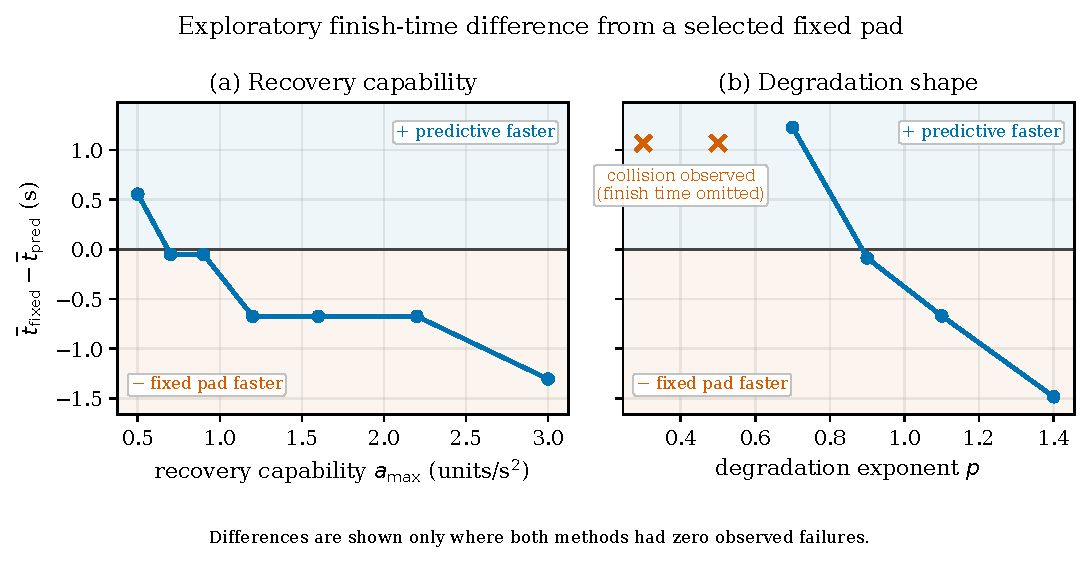
\includegraphics[width=\columnwidth]{fig_boundary.pdf}
  \caption{Exploratory elapsed-time difference between the selected fixed pad
  and the $T_h=2.0$\,s predictive rule across (a) recovery capability and (b)
  degradation shape at $a_{\max}=0.8$.  Positive values favor prediction.
  Differences are shown only where both rules recorded no failure; crosses mark
  settings in which the predictive rule collides and no tested fixed pad
  succeeds in every episode.}
  \label{fig:boundary}
\end{figure}

\subsection{Seed-Disjoint Single-Margin Evaluation}

The equal-budget searches select $\rho=2.5$\,s and $T_h=2.5$\,s
(\cref{tab:single-margin}).  On the 6,750 held-out conflict episodes, the fixed
rule succeeds in all episodes and records no collision.  The tuned predictive
rule succeeds in 6,748 and records two collisions, one at each of the two highest
severities with $a_{\max}=0.5$ and $p=0.7$.  Its successful-only mean elapsed
time is $26.577$\,s, compared with $27.690$\,s for the fixed rule, but these
means condition on different success sets.  We therefore attach no paired
interval and claim no efficiency advantage.  For context, the retained
$T_h=2.0$\,s rule records 172 collisions on the same held-out set.

\begin{table}[!t]
  \centering
  \caption{Seed-Disjoint Single-Margin Test Results over 6,750 Conflict
  Episodes per Arm}
  \label{tab:single-margin}
  \footnotesize
  \setlength{\tabcolsep}{3.5pt}
  \begin{tabular}{@{}llrrr@{}}
    \toprule
    Rule & Parameter & Collisions & Successes & Mean time (s) \\
    \midrule
    Fixed pad, tuned & $\rho=2.5$\,s & 0 & 6,750 & 27.690 \\
    Predictive, tuned & $T_h=2.5$\,s & 2 & 6,748 & 26.577 \\
    Predictive, retained & $T_h=2.0$\,s & 172 & 6,578 & 25.990 \\
    \bottomrule
  \end{tabular}

  \vspace{3pt}
  \parbox{\columnwidth}{\scriptsize Mean elapsed time is averaged over
  successful episodes only and therefore conditions on different success sets
  for different rules.}
\end{table}


In the 2,250 held-out clear episodes, both tuned rules complete without
collision.  The fixed rule yields unnecessarily in $1800/2250$ episodes
(80.0\%), and the predictive rule in $1358/2250$ (60.4\%).  This is evidence of
fewer interventions on the specified clear grid, not a safety-adjusted
performance gain.  The largest upper endpoint of the pointwise 95\% Wilson
collision intervals is $0.025$ for the fixed rule and $0.037$ for the
predictive rule.

\subsection{Seed-Disjoint Coordination Evaluation}

The redesigned geometry first passes a falsification check: without
intervention, all 1,620 held-out conflict runs reach the exit but contain both a
zone-occupancy collision and a headway violation, so none succeeds
(\cref{tab:coordination}).  These runs consume no measurement noise and are
therefore deterministic repeats within each physical scenario; their count
verifies coverage of the grid, not 1,620 independent safety trials.

\begin{table}[!t]
  \centering
  \caption{Seed-Disjoint Coordination Test Results over 1,620 Episodes per Rule
  and Condition}
  \label{tab:coordination}
  \footnotesize
  \setlength{\tabcolsep}{4pt}
  \newcommand{\armhead}[2]{\begin{tabular}[b]{@{}c@{}}#1\\#2\end{tabular}}
  \begin{tabular}{@{}lrrr@{}}
    \toprule
    & \armhead{No}{intervention} & \armhead{Fixed pad}{$\rho=1.75$\,s}
      & \armhead{Predictive}{$T_h=1.50$\,s} \\
    \midrule
    \multicolumn{4}{@{}l}{\textit{Conflict condition}} \\
    Successful episodes        & 0      & 1,620  & 1,620  \\
    Collisions                 & 1,620  & 0      & 0      \\
    Headway violations         & 1,620  & 0      & 0      \\
    Mean makespan (s)          & --     & 29.813 & 27.034 \\
    Mean first trigger (s)     & --     & 4.534  & 5.917  \\
    \addlinespace[2pt]
    \multicolumn{4}{@{}l}{\textit{Clear condition}} \\
    Successful episodes        & 1,620  & 1,620  & 1,620  \\
    Serializations             & 0      & 1,080  & 21     \\
    Mean makespan (s)          & 20.000 & 26.337 & 20.278 \\
    \bottomrule
  \end{tabular}

  \vspace{3pt}
  \parbox{\columnwidth}{\scriptsize Makespan is averaged over successful
  episodes.  No rule records a timeout, repeated yield, or serialization breach.
  The paired fixed-minus-predictive conflict difference is $2.779$\,s, with a
  95\% interval of $[2.659,2.902]$\,s from a bootstrap clustered by test
  replicate.}
\end{table}


The searches select $\rho=1.75$\,s and $T_h=1.50$\,s, each with 540 of 540
successful tuning episodes and no serialization breach.  Each selected rule then
succeeds in all 1,620 held-out conflict episodes with no collision, headway
violation, timeout, repeated yield, or serialization breach.  The mean
successful makespan is $29.813$\,s for the fixed rule and $27.034$\,s for the
predictive rule, whose mean first trigger occurs later ($5.917$ versus
$4.534$\,s) and so avoids some waiting without changing the observed success
count.  The paired fixed-minus-predictive difference is $2.779$\,s, with a 95\%
interval of $[2.659,2.902]$\,s from a bootstrap that clusters the 27-scenario
grid by the 60 test replicates.  This is an efficiency comparison at matched
observed outcomes, conditional on the modeled scenarios and noise distribution.

In the clear condition, every run without intervention succeeds in $20.000$\,s,
and both selected rules also succeed in all 1,620 episodes.  The fixed rule
commits an unnecessary serialization in $1080/1620$ episodes (66.7\%) and has a
mean makespan of $26.337$\,s; the predictive rule serializes in $21/1620$
(1.3\%) and has a mean of $20.278$\,s.  No interval was computed for this
clear-path difference, so it remains descriptive.

\section{Discussion}\label{sec:disc}

Before implementing prediction, one can first ask whether its lead changes what recovery can accomplish. Prediction is most plausible when recovery is slow enough for an earlier trigger to cross the boundary in Proposition~\ref{prop:boundary}, and when degradation rates vary in a way that can be estimated before that boundary. At one known constant rate, a fixed pad reproduces the studied predictive trigger. Under fast, committed serialization, tuning may remove predictive lead altogether.

The simulators produce different results. In the single-margin study, the exploratory figures favor prediction over the unpadded rules and, in a few settings, over the in-sample fixed pad. After equal-budget, seed-disjoint tuning, the predictive arm intervenes less often on clear paths and has a lower descriptive successful-only elapsed time. It also records two held-out conflict collisions where the fixed arm records none, so an efficiency comparison at matched outcomes is unavailable. In the coordination study, both tuned arms succeed throughout the held-out conflict grid and the predictive arm finishes earlier. Its lower rate of clear-path serialization is consistent with adaptation to degradation rate.

The coordination result depends on the recovery design. The first trigger commits one total order, after which blockers and release events determine the motion. Prediction changes when this commitment occurs; the order is never revised. The paired interval thus describes variation over measurement noise on the fixed 27-scenario grid. It says nothing about unseen geometries, robot counts, dynamics, or online re-planning.

Proposition~\ref{prop:reduction} also suggests an intermediate design: scale a current-margin threshold using an online rate estimate, without constructing a larger predict-then-recover stack. Its practical value would still depend on estimator delay, noise, and changes in degradation rate.

Zero observed collisions is not a safety guarantee. The pointwise Wilson intervals are not simultaneous bounds over the scenario family, and holding out noise seeds does not create a new population of robot environments. The v1 comparison accordingly tunes the simpler early-trigger baseline, verifies that untreated paths conflict, separates tuning from testing, and reports failures before conditional timing.

\section{What I take from this}
\label{sec:conclusion}

For the trigger studied here, prediction is a way to adapt a margin threshold
to the estimated rate of decline.  Its value depends on whether the extra lead
changes what recovery can accomplish and how much unnecessary early action it
avoids.  In the timing model, recovery duration and deadline slack set that
boundary, and observation age consumes the available lead one for one.

The three-robot experiment shows a practical benefit of this adaptation.  Both
tuned rules succeed in all 1,620 conflict episodes, while prediction reduces
mean completion time by $2.779$\,s (paired 95\% interval
$[2.659,2.902]$\,s).  It also cuts unnecessary clear-path serializations from
1,080 to 21 out of 1,620 episodes.  Waiting until closer to the point when
recovery is needed saves time in this fixed-order crossing setup.

The two-robot experiment shows why the rate estimate matters.  The tuned fixed
rule records $0/6750$ conflict collisions and prediction records $2/6750$, both
where the conflict is revealed late and braking is slow.  A rate estimate that
lags a steepening decline can use up the lead the predictive rule was meant to
provide.

My takeaway is that the recovery requirement is the right place to start.
When recovery needs similar lead times across cases but margins decline at
different rates, adapting the threshold can reduce unnecessary waiting.
Observation delay and changing recovery durations are the next variables I
would test, using the tuned fixed threshold as the baseline.

\emph{Code and data.}  The simulators, tests, episode-level results, and figure
scripts are available at \url{\repositoryurl}.


\bibliographystyle{IEEEtran}
\bibliography{references}

\end{document}
